%\documentclass{beamer}
%\usetheme{Pittsburgh}
\documentclass{scrartcl}

\usepackage[utf8]{inputenc}
\usepackage{default}
\usepackage[procnames]{listings}
\usepackage{graphicx}
%\usepackage[toc,page]{appendix}
\usepackage{caption}
\usepackage{hyperref}
\usepackage{color}
%\usepackage{csvsimple}
\usepackage{float}
\usepackage[T1]{fontenc}



%Bibliogrpahy?
%\usepackage{bibentry}
%\nobibliography*
%\bibentry{ }


%Python
\definecolor{keywords}{RGB}{255,0,90}
\definecolor{comments}{RGB}{0,0,113}
\definecolor{red}{RGB}{160,0,0}
\definecolor{green}{RGB}{0,150,0}
\lstset{language=Python,
    basicstyle=\ttfamily\scriptsize,
    keywordstyle=\color{keywords},
    commentstyle=\color{comments},
    stringstyle=\color{red},
    identifierstyle=\color{green},
    breaklines = true,
    columns=fullflexible,
    %Numbering and tabs
    %numbers=left,
    %numberstyle=\tiny\color{gray},
    %stepnumber=2,
    %numbersep=1em,
    tabsize=4,
    showspaces=false,
    showstringspaces=false}

\begin{document}

\title{Learning and Adaptivity}
\subtitle{Report No. 2}
\author{
  \href{daiem.ali@smail.inf.h-brs.de}{Ali, Daiem}: \href{https://github.com/daiemna}{github.com/daiemna}\\
  \href{christophe.quignon@smail.inf.h-brs.de}{Quignon, Christophe}:\href{https://github.com/ChrisQuignon}{github.com/ChrisQuignon}
  %Familyname, Name
}
\date{\today}


\maketitle

%TODO: add abstract and conclusion
%labels (or zero)
%references (or zero)
%remove scaffolding code


\begin{abstract}
The abstract goes here
\end{abstract}


\section{Project introduction}
%Include an introduction section to your project

%Subject
%Method
%justification

\section{Features}
% Include information on which features are available from your data, and include visualizations


\begin{figure}[H]
  \centering
  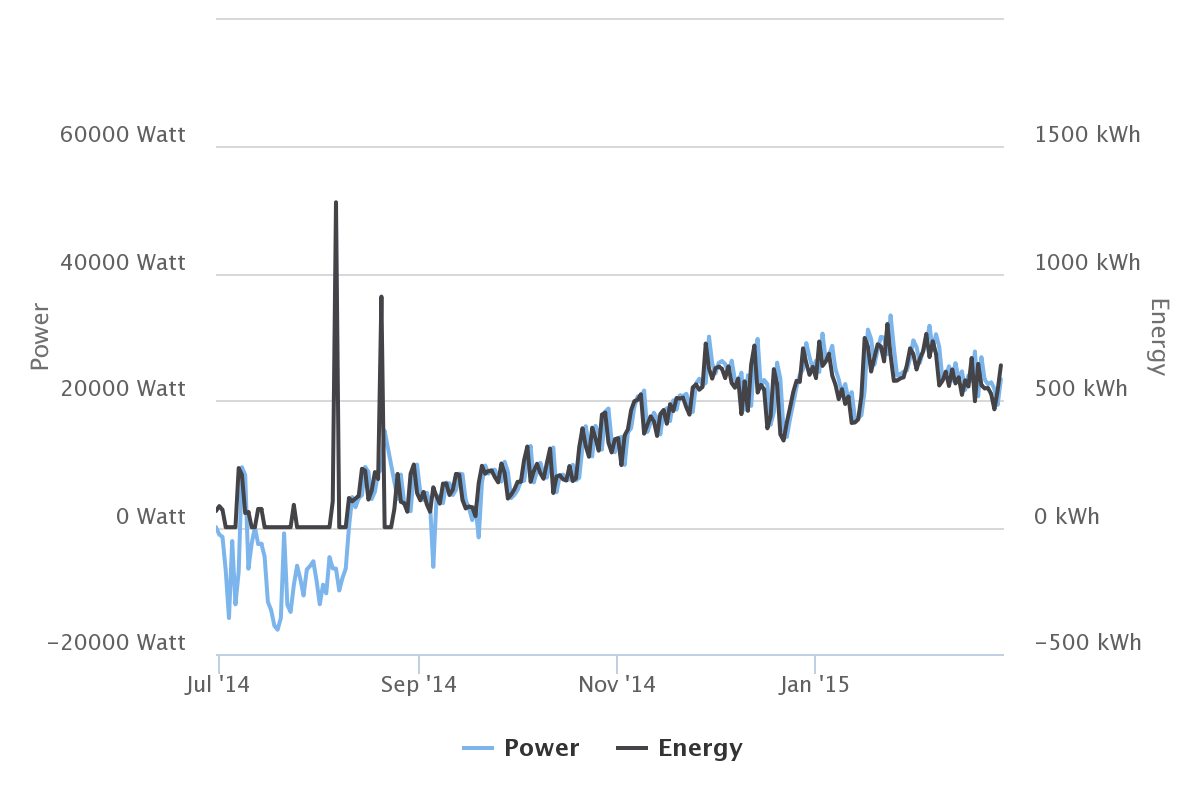
\includegraphics[width=0.8\linewidth]{img/powerenergy.png}
  %TODO add caption
  \caption{}
  %\label{fig:}
\end{figure}

\begin{figure}[H]
  \centering
  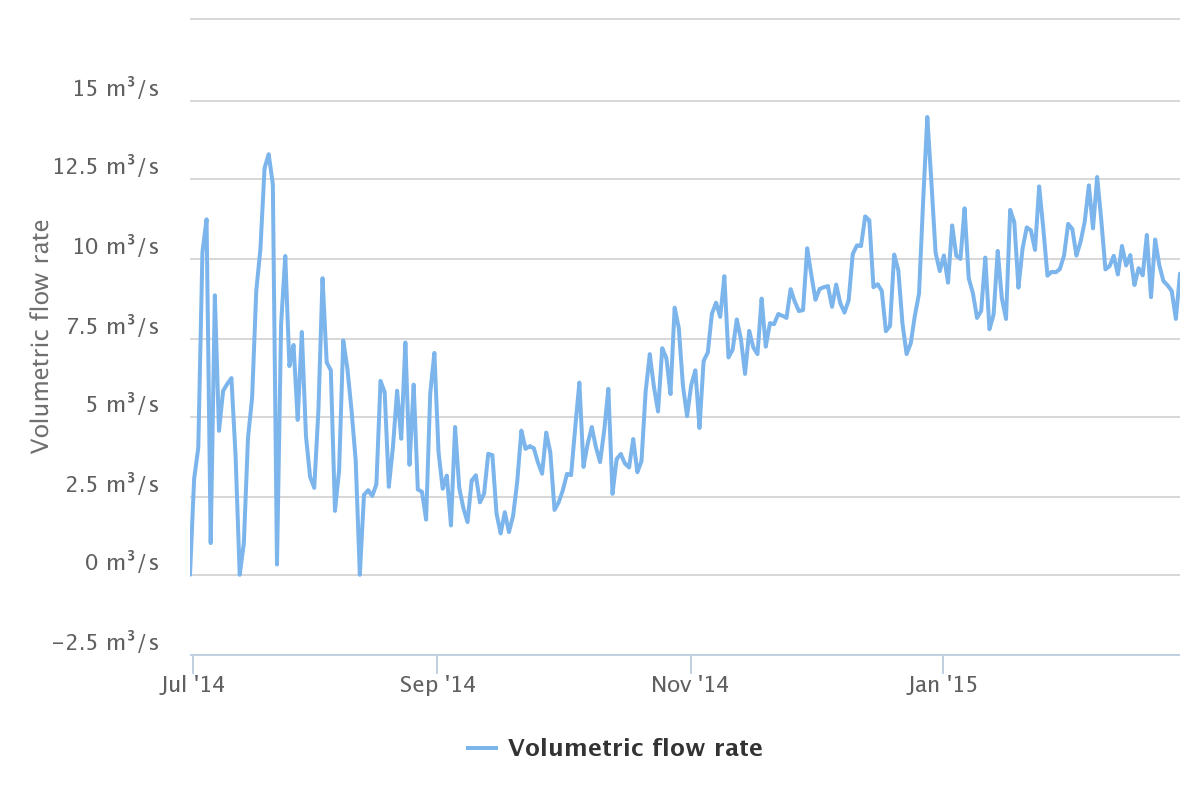
\includegraphics[width=0.8\linewidth]{img/Volumetric_flow.png}
  %TODO add caption
  \caption{}
  %\label{fig:}
\end{figure}

\begin{figure}[H]
  \centering
  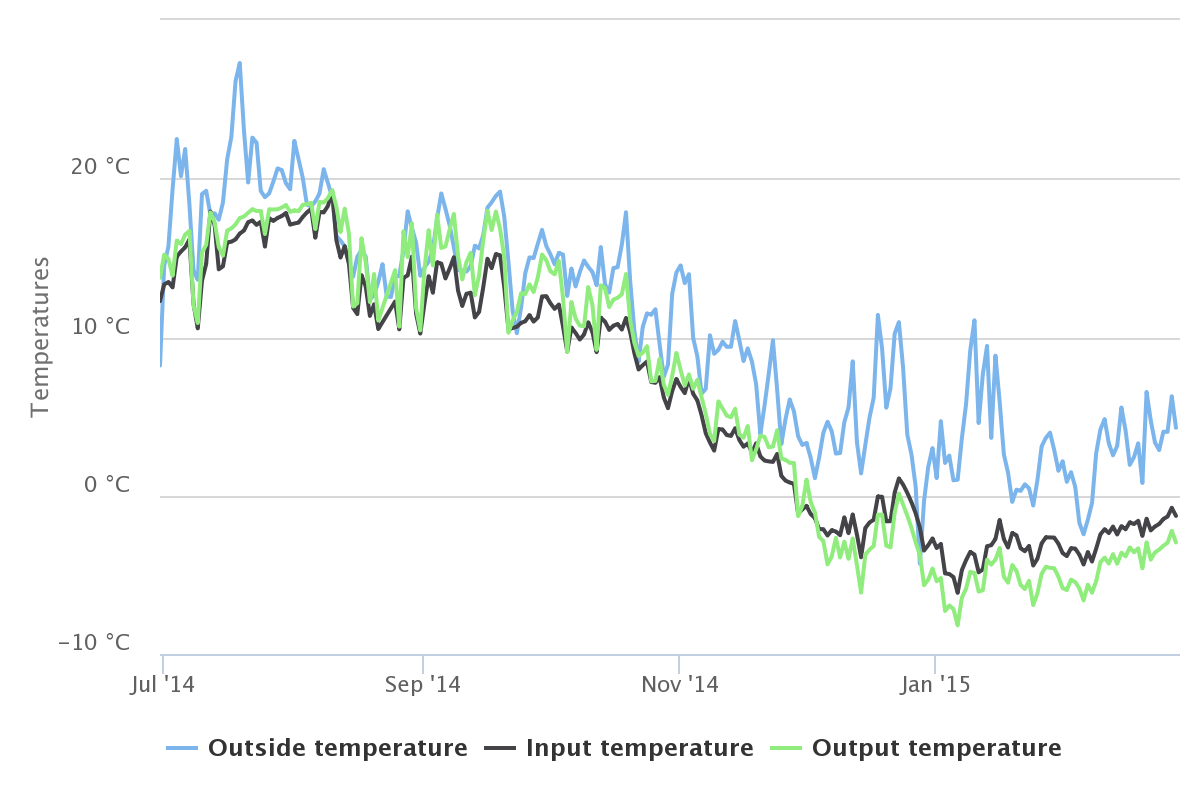
\includegraphics[width=0.8\linewidth]{img/Temperatures.png}
  %TODO add caption
  \caption{}
  %\label{fig:}
\end{figure}

\begin{figure}[H]
  \centering
  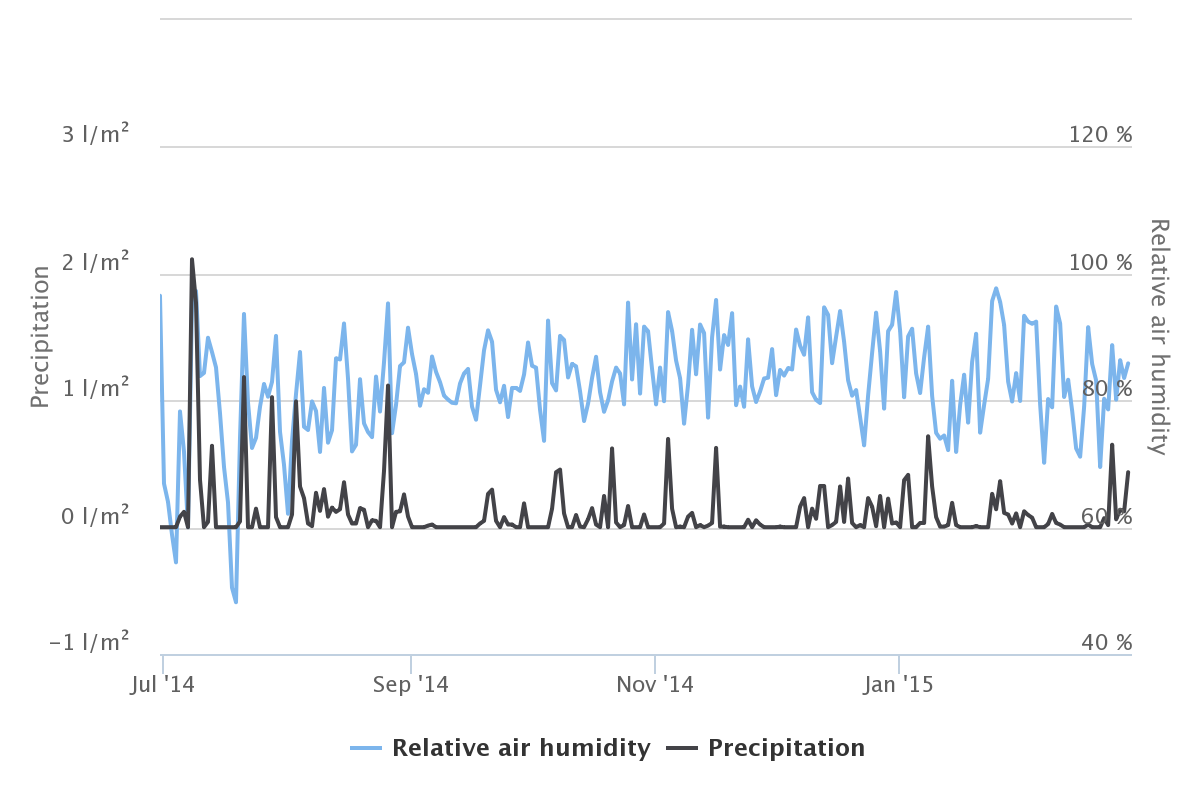
\includegraphics[width=0.8\linewidth]{img/humidity.png}
  %TODO add caption
  \caption{}
  %\label{fig:}
\end{figure}


\section{Method}
%Include a section on what Machine Learning method you intend to use, and why you believe it will be suitable for your data.

\section{Conclusion} 
%haha\cite{kumar2006forecasting}


%BIBLIOGRPAHY?
\bibliographystyle{plain}%amsalpha
\bibliography{bib.bib}
%\bibentry{}

\begin{appendix}
\section{}

\end{appendix}


%COPY AND PASTE FROM HERE

%\begin{enumerate}
% \item
%\end{enumerate}

%\href{link}{text}

%\begin[Language=Python]{lstlisting}
%#PYTHON CODE HERE
%\end{lstlisting}

%\lstinputlisting[language=Python]{	}

%\csvautotabular[separator=semicolon]{data.csv}

%\subsubsection{left}
%\begin{figure}[H]
%  \centering
%  \includegraphics[width=0.5\linewidth]{../img/	}
%  %\caption{}
%  %\label{fig:}
%\end{figure}
%PUT UNITS ON THE FIGURES

\end{document}
